\documentclass{article}
\usepackage[main]{neurips_2026}
\usepackage[utf8]{inputenc}
\usepackage[T1]{fontenc}
\usepackage{hyperref,url,booktabs,amsmath,amssymb,amsthm,graphicx,microtype,xcolor}
\newtheorem{theorem}{Theorem}
\newtheorem{corollary}{Corollary}
\newtheorem{lemma}{Lemma}
\newcommand{\R}{\mathbb R}
\newcommand{\num}[1]{\csname #1\endcsname}
% Generated by src/report.py; do not edit.
\expandafter\def\csname ArenaN\endcsname{57,477}
\expandafter\def\csname ArenaM\endcsname{64}
\expandafter\def\csname ArenaK\endcsname{2}
\expandafter\def\csname ArenaResolutionK\endcsname{27}
\expandafter\def\csname ArenaLowerK\endcsname{2}
\expandafter\def\csname ArenaLeaderN\endcsname{7387}
\expandafter\def\csname ArenaDirectCapacity\endcsname{31}
\expandafter\def\csname ArenaGap\endcsname{0.008}
\expandafter\def\csname ArenaGapLo\endcsname{-0.097}
\expandafter\def\csname ArenaGapHi\endcsname{0.116}
\expandafter\def\csname ArenaGlobalPct\endcsname{0.0035}
\expandafter\def\csname ArenaLeaderPct\endcsname{0.03}
\expandafter\def\csname ArenaBootReverse\endcsname{44.2}
\expandafter\def\csname MThumanN\endcsname{3,355}
\expandafter\def\csname MThumanM\endcsname{6}
\expandafter\def\csname MThumanK\endcsname{46}
\expandafter\def\csname MThumanResolutionK\endcsname{78}
\expandafter\def\csname MThumanLowerK\endcsname{46}
\expandafter\def\csname MThumanLeaderN\endcsname{1029}
\expandafter\def\csname MThumanDirectCapacity\endcsname{91}
\expandafter\def\csname MThumanGap\endcsname{0.376}
\expandafter\def\csname MThumanGapLo\endcsname{0.124}
\expandafter\def\csname MThumanGapHi\endcsname{0.654}
\expandafter\def\csname MThumanGlobalPct\endcsname{1.3711}
\expandafter\def\csname MThumanLeaderPct\endcsname{4.47}
\expandafter\def\csname MThumanBootReverse\endcsname{0.2}
\expandafter\def\csname MTGPTFourN\endcsname{2,400}
\expandafter\def\csname MTGPTFourM\endcsname{6}
\expandafter\def\csname MTGPTFourK\endcsname{61}
\expandafter\def\csname MTGPTFourResolutionK\endcsname{93}
\expandafter\def\csname MTGPTFourLowerK\endcsname{61}
\expandafter\def\csname MTGPTFourLeaderN\endcsname{800}
\expandafter\def\csname MTGPTFourDirectCapacity\endcsname{75}
\expandafter\def\csname MTGPTFourGap\endcsname{0.809}
\expandafter\def\csname MTGPTFourGapLo\endcsname{0.480}
\expandafter\def\csname MTGPTFourGapHi\endcsname{1.090}
\expandafter\def\csname MTGPTFourGlobalPct\endcsname{2.5417}
\expandafter\def\csname MTGPTFourLeaderPct\endcsname{7.62}
\expandafter\def\csname MTGPTFourBootReverse\endcsname{0.0}
\expandafter\def\csname NBA2010N\endcsname{1,230}
\expandafter\def\csname NBA2010M\endcsname{30}
\expandafter\def\csname NBA2010K\endcsname{2}
\expandafter\def\csname NBA2010ResolutionK\endcsname{13}
\expandafter\def\csname NBA2010LowerK\endcsname{2}
\expandafter\def\csname NBA2010LeaderN\endcsname{82}
\expandafter\def\csname NBA2010DirectCapacity\endcsname{2}
\expandafter\def\csname NBA2010Gap\endcsname{0.117}
\expandafter\def\csname NBA2010GapLo\endcsname{-0.503}
\expandafter\def\csname NBA2010GapHi\endcsname{0.772}
\expandafter\def\csname NBA2010GlobalPct\endcsname{0.1626}
\expandafter\def\csname NBA2010LeaderPct\endcsname{2.44}
\expandafter\def\csname NBA2010BootReverse\endcsname{36.0}
\expandafter\def\csname NBA2011N\endcsname{1,230}
\expandafter\def\csname NBA2011M\endcsname{30}
\expandafter\def\csname NBA2011K\endcsname{1}
\expandafter\def\csname NBA2011ResolutionK\endcsname{11}
\expandafter\def\csname NBA2011LowerK\endcsname{1}
\expandafter\def\csname NBA2011LeaderN\endcsname{82}
\expandafter\def\csname NBA2011DirectCapacity\endcsname{1}
\expandafter\def\csname NBA2011Gap\endcsname{0.062}
\expandafter\def\csname NBA2011GapLo\endcsname{-0.676}
\expandafter\def\csname NBA2011GapHi\endcsname{0.722}
\expandafter\def\csname NBA2011GlobalPct\endcsname{0.0813}
\expandafter\def\csname NBA2011LeaderPct\endcsname{1.22}
\expandafter\def\csname NBA2011BootReverse\endcsname{40.0}
\expandafter\def\csname NBA2012N\endcsname{990}
\expandafter\def\csname NBA2012M\endcsname{30}
\expandafter\def\csname NBA2012K\endcsname{2}
\expandafter\def\csname NBA2012ResolutionK\endcsname{11}
\expandafter\def\csname NBA2012LowerK\endcsname{1}
\expandafter\def\csname NBA2012LeaderN\endcsname{66}
\expandafter\def\csname NBA2012DirectCapacity\endcsname{0}
\expandafter\def\csname NBA2012Gap\endcsname{0.106}
\expandafter\def\csname NBA2012GapLo\endcsname{-0.663}
\expandafter\def\csname NBA2012GapHi\endcsname{0.895}
\expandafter\def\csname NBA2012GlobalPct\endcsname{0.2020}
\expandafter\def\csname NBA2012LeaderPct\endcsname{3.03}
\expandafter\def\csname NBA2012BootReverse\endcsname{34.4}
\expandafter\def\csname NBA2013N\endcsname{1,229}
\expandafter\def\csname NBA2013M\endcsname{30}
\expandafter\def\csname NBA2013K\endcsname{3}
\expandafter\def\csname NBA2013ResolutionK\endcsname{14}
\expandafter\def\csname NBA2013LowerK\endcsname{3}
\expandafter\def\csname NBA2013LeaderN\endcsname{82}
\expandafter\def\csname NBA2013DirectCapacity\endcsname{2}
\expandafter\def\csname NBA2013Gap\endcsname{0.279}
\expandafter\def\csname NBA2013GapLo\endcsname{-0.292}
\expandafter\def\csname NBA2013GapHi\endcsname{0.963}
\expandafter\def\csname NBA2013GlobalPct\endcsname{0.2441}
\expandafter\def\csname NBA2013LeaderPct\endcsname{3.66}
\expandafter\def\csname NBA2013BootReverse\endcsname{16.4}
\expandafter\def\csname NBA201FourN\endcsname{1,230}
\expandafter\def\csname NBA201FourM\endcsname{30}
\expandafter\def\csname NBA201FourK\endcsname{4}
\expandafter\def\csname NBA201FourResolutionK\endcsname{17}
\expandafter\def\csname NBA201FourLowerK\endcsname{2}
\expandafter\def\csname NBA201FourLeaderN\endcsname{82}
\expandafter\def\csname NBA201FourDirectCapacity\endcsname{0}
\expandafter\def\csname NBA201FourGap\endcsname{0.185}
\expandafter\def\csname NBA201FourGapLo\endcsname{-0.474}
\expandafter\def\csname NBA201FourGapHi\endcsname{0.819}
\expandafter\def\csname NBA201FourGlobalPct\endcsname{0.3252}
\expandafter\def\csname NBA201FourLeaderPct\endcsname{4.88}
\expandafter\def\csname NBA201FourBootReverse\endcsname{33.4}
\expandafter\def\csname NBA2015N\endcsname{1,230}
\expandafter\def\csname NBA2015M\endcsname{30}
\expandafter\def\csname NBA2015K\endcsname{8}
\expandafter\def\csname NBA2015ResolutionK\endcsname{21}
\expandafter\def\csname NBA2015LowerK\endcsname{5}
\expandafter\def\csname NBA2015LeaderN\endcsname{82}
\expandafter\def\csname NBA2015DirectCapacity\endcsname{1}
\expandafter\def\csname NBA2015Gap\endcsname{0.546}
\expandafter\def\csname NBA2015GapLo\endcsname{-0.192}
\expandafter\def\csname NBA2015GapHi\endcsname{1.203}
\expandafter\def\csname NBA2015GlobalPct\endcsname{0.6504}
\expandafter\def\csname NBA2015LeaderPct\endcsname{9.76}
\expandafter\def\csname NBA2015BootReverse\endcsname{6.4}
\expandafter\def\csname MatchedhumanN\endcsname{1,814}
\expandafter\def\csname MatchedhumanM\endcsname{6}
\expandafter\def\csname MatchedhumanK\endcsname{20}
\expandafter\def\csname MatchedhumanResolutionK\endcsname{36}
\expandafter\def\csname MatchedhumanLowerK\endcsname{20}
\expandafter\def\csname MatchedhumanLeaderN\endcsname{578}
\expandafter\def\csname MatchedhumanDirectCapacity\endcsname{51}
\expandafter\def\csname MatchedhumanGap\endcsname{0.283}
\expandafter\def\csname MatchedhumanGapLo\endcsname{0.066}
\expandafter\def\csname MatchedhumanGapHi\endcsname{0.496}
\expandafter\def\csname MatchedhumanGlobalPct\endcsname{1.1025}
\expandafter\def\csname MatchedhumanLeaderPct\endcsname{3.46}
\expandafter\def\csname MatchedhumanBootReverse\endcsname{0.6}
\expandafter\def\csname MatchedGPTFourN\endcsname{1,814}
\expandafter\def\csname MatchedGPTFourM\endcsname{6}
\expandafter\def\csname MatchedGPTFourK\endcsname{42}
\expandafter\def\csname MatchedGPTFourResolutionK\endcsname{68}
\expandafter\def\csname MatchedGPTFourLowerK\endcsname{42}
\expandafter\def\csname MatchedGPTFourLeaderN\endcsname{578}
\expandafter\def\csname MatchedGPTFourDirectCapacity\endcsname{55}
\expandafter\def\csname MatchedGPTFourGap\endcsname{0.759}
\expandafter\def\csname MatchedGPTFourGapLo\endcsname{0.441}
\expandafter\def\csname MatchedGPTFourGapHi\endcsname{1.107}
\expandafter\def\csname MatchedGPTFourGlobalPct\endcsname{2.3153}
\expandafter\def\csname MatchedGPTFourLeaderPct\endcsname{7.27}
\expandafter\def\csname MatchedGPTFourBootReverse\endcsname{0.0}
\expandafter\def\csname Repeats\endcsname{500}
\expandafter\def\csname BootstrapRepeats\endcsname{500}
\expandafter\def\csname Seed\endcsname{20261102}
\expandafter\def\csname MatchedRepeats\endcsname{100}
\expandafter\def\csname MainSeconds\endcsname{95.0}
\expandafter\def\csname WinnerSeconds\endcsname{11.0}
\expandafter\def\csname PeakMiB\endcsname{344.7}
\expandafter\def\csname AdjacentCount\endcsname{83}
\expandafter\def\csname AdjacentTight\endcsname{72}
\expandafter\def\csname AdjacentExactPrediction\endcsname{65}
\expandafter\def\csname AdjacentMAE\endcsname{0.73}
\expandafter\def\csname AdjacentMaxError\endcsname{9}
\expandafter\def\csname MatchedHumanMin\endcsname{15}
\expandafter\def\csname MatchedHumanMax\endcsname{26}
\expandafter\def\csname MatchedHumanMedian\endcsname{20}
\expandafter\def\csname ArenaAdjacentMax\endcsname{104}
\expandafter\def\csname MainWinnerExact\endcsname{6}
\expandafter\def\csname MainPairExact\endcsname{6}

\title{Exact and Bounded Stability Audits for Pairwise Leaderboards}
\author{Anonymous Research Artifact}
\begin{document}
\maketitle
\begin{abstract}
A small number of changed comparisons can reverse a leaderboard, but the meaning of ``small'' depends on score separation, exposure, and the perturbation model. We audit fixed-schedule outcome reversals in ridge Bradley--Terry rankings across crowdsourced preferences, expert judgments, model judgments, and basketball results. A direct-transfer relaxation gives a finite-edit lower bound: no set of $k$ outcome reversals reduces a queried score gap more than $k$ unconstrained transfers between its endpoints. When enough appropriate direct comparisons exist, the bound is attainable and the minimum reversal budget is exact. Across nine main panels, we certify the exact winner-change budget in \num{MainWinnerExact}. These budgets include \num{ArenaK} records for the Arena snapshot and \num{MThumanK} and \num{MTGPTFourK} for expert and GPT-4 judgments. Arena's leading gap is already unresolved under resampling; its two-edit threshold becomes \num{ArenaResolutionK} for a reversal beyond twice its original bootstrap standard deviation. Matching judgment schedules preserves a larger GPT-4 threshold in these data. We find substantial variation within designs, and show why global edit percentages, participant exposure, and sampling uncertainty must be reported together.
\end{abstract}

\section{Introduction}
Pairwise leaderboards turn comparisons into consequential ordinal statements: which model to deploy, which release is ahead, or which team is strongest. In preference evaluation, the observations are judgments rather than ground truth. Chatbot Arena gathers anonymous user comparisons and estimates model strengths from them \citep{chiang2024arena}; MT-Bench offers expert and model-generated judgments on a controlled question set \citep{zheng2023judge}. The same mathematical ranking model also applies to sporting outcomes. An ordering can change because a close contest is intrinsically uncertain, because a participant has little supporting data, or because particular observations have disproportionate influence. These mechanisms should not be conflated.

Our question is operational: \emph{with the observed comparison schedule fixed, how many decisive outcomes must be reversed to change an estimated order, and how does that budget compare with random noise, participant exposure, and sampling uncertainty?} We study offline data sensitivity. The ability to rewrite arbitrary historical records is stronger than a practical voter's access. A reversal budget is consequently an audit of an estimator and dataset, not an estimate of the effort required to compromise a live service.

We distinguish the reversal of the original leading pair from the loss of the original winner to \emph{any} competitor. Searching for a successful edit set gives an upper bound on the optimal budget, not evidence that fewer edits are impossible. We derive a complementary lower bound for the standard ridge Bradley--Terry model. Its Hessian is a comparison-graph Laplacian plus a positive diagonal. A maximum principle implies that a direct transfer between the queried participants is the most effective unit transfer at every parameter value. Integrating this fact gives a global comparison with a virtual, capacity-free direct-transfer path. Sufficient recorded direct wins make the relaxation attainable; otherwise we retain a lower/upper interval.

The empirical study uses a fixed Arena snapshot, both MT-Bench judgment panels, and the last six complete calendar-labeled NBA seasons in the supplied historical archive. It also uses a matched MT-Bench schedule, multiple perturbation baselines, cluster resampling, and modeling controls. We obtain exact or bounded answers rather than presenting a heuristic attack count as a universal robustness metric.

Three findings guide interpretation. First, the Arena leading pair is exceptionally close: its gap is \num{ArenaGap}, with a bootstrap interval $[\num{ArenaGapLo},\num{ArenaGapHi}]$. A tiny point-order reversal is therefore a different event from overturning a well-separated result. Second, the denominator matters. NBA teams contribute a much smaller share of their board's comparisons than models do in the six-model MT-Bench panels; counting all records makes those differences look larger. Third, matching the human and GPT-4 schedules preserves the observed difference in leading-pair robustness, but cannot establish that a judge type is inherently better. Stability can also preserve systematic preferences or bias.

\section{Related work}
\citet{chiang2024arena} describe preference collection, Bradley--Terry estimation, uncertainty, and sampling design in Chatbot Arena. \citet{zheng2023judge} compare expert and LLM judgments, including order inconsistency and self-enhancement bias. These studies motivate comparing evaluation designs while avoiding the assumption that a more decisive judge is a more valid one.

Our candidate-selection baseline follows the general influence-function approach of \citet{koh2017influence}: differentiate a fitted optimum through its estimating equations. \citet{broderick2023robustness} use influence approximations to find influential deletions and emphasize exact refitting and the distinction between sampling uncertainty and sensitivity to selected subsets. We use this distinction directly. Our label-reversal threat leaves the comparison graph unchanged, whereas deletion changes both its weights and its outcomes. We report both operations but do not equate their budgets.

\citet{min2025rigging} study new-vote manipulation in Arena, including effects through comparisons that do not involve the target. Our contribution is not the observation that pairwise rankings can be manipulated. We analyze a fixed-schedule historical-edit model, derive a finite-edit lower bound with an attainability test, and compare its consequences across real evaluation designs with exposure and uncertainty controls. The theorem applies to item-only ridge Bradley--Terry fits; it does not claim optimality for new-vote collection, arbitrary covariates, or deletions. To preserve the requested independent research boundary, literature access was confined to selected supplied starting references and dataset documentation; this is not an exhaustive literature review.

\section{Audit model and finite-edit bounds}
\label{sec:method}
\subsection{Estimator, edits, and endpoints}
Record $r$ compares items $a_r,b_r$, with $x_r=e_{a_r}-e_{b_r}$ and outcome $y_r\in\{0,1/2,1\}$. A tie contributes one half-win observation, with the same total loss weight as a decisive record. The fitted score vector is
\begin{equation}
 \hat\theta=\arg\min_{\theta\in\R^M}F(\theta),\quad
 F(\theta)=\sum_{r=1}^N\big[\log(1+e^{x_r^\top\theta})-y_rx_r^\top\theta\big]
       +\frac{\lambda}{2}\|\theta\|_2^2. \label{eq:model}
\end{equation}
We use natural-logit scores, $\lambda=1$ on the \emph{summed} loss, and controls at $0.1$ and $10$. Positive ridge makes every fit unique even after unfavorable edits; it also affects very close rankings. Scores sum to zero automatically. These are our standardized reconstructed boards, not replicas of any current platform's production leaderboard.

An eligible edit reverses one originally decisive record, $y_r\mapsto1-y_r$, once. It preserves participants, schedule, and $N$; ties are not editable. For an edit set $E$,
\begin{equation}
 F_E(\theta)=F(\theta)+b_E^\top\theta,\qquad
 b_E=\sum_{r\in E}(2y_r-1)x_r
     =\sum_{r\in E}(e_{w_r}-e_{l_r}). \label{eq:edit}
\end{equation}
Here $w_r,l_r$ are the original winner and loser. Fix the original leader $\ell$ and runner-up $r_0$, and put $c=e_\ell-e_{r_0}$ and $\hat\Delta=c^\top\hat\theta>0$. Our primary pair endpoint is a strict reversal, $c^\top\hat\theta_E<0$. Let $K^*_{\ell r_0}$ be its minimum feasible edit count. Separately, $K^*_{\rm win}=\min_{j\ne\ell}K^*_{\ell j}$ measures loss to any competitor. Exact score ties do not count as reversals.

We report $k$, $k/N$, and $k/n_\ell$, where $n_\ell$ is the number of original records involving the leader, including ties. The last is an exposure scale, not a probability or a claim that all edits must touch the leader. For the reported leading-pair static paths, all selected edits do touch it. None of these denominators equates human effort, corruption probability, or information across domains.

\subsection{A direct-transfer relaxation}
For $t\ge0$ define the virtual fit
\begin{equation}
 \theta_c(t)=\arg\min_\theta\{F(\theta)+t c^\top\theta\},\quad
 L_c=\min\{k\in\mathbb N:c^\top\theta_c(k)<0\}. \label{eq:virtual}
\end{equation}
The virtual path can transfer more wins than were observed, even when the pair never met. It is a mathematical relaxation, not generated evidence. Strong convexity makes these virtual fits well-defined.

\begin{theorem}[Direct-transfer domination]
\label{thm:direct}
Under Eq.~\eqref{eq:model} with $\lambda>0$, item effects only, and the fixed-schedule reversal model in Eq.~\eqref{eq:edit}, for every set $E$ of $k$ eligible edits and any contrast $c=e_i-e_j$,
\begin{equation}
 c^\top\hat\theta_E\ \ge\ c^\top\theta_c(k). \label{eq:domination}
\end{equation}
Consequently $K^*_{ij}\ge L_c$. If at least $L_c$ recorded decisive outcomes are wins by $i$ against $j$, then $K^*_{ij}=L_c$.
\end{theorem}
\noindent\emph{Proof sketch.} Write $H(\theta)=L(\theta)+\lambda I$ where $L$ is a graph Laplacian with nonnegative logistic curvature weights. The solution $v=H(\theta)^{-1}c$ has its maximum at $i$ and its minimum at $j$. Hence $v^\top(e_w-e_l)\le v^\top c$ for every possible outcome direction. Interpolate the linear perturbation from $b_E$ to $kc$ and differentiate its optimum. The queried gap cannot increase along that interpolation, proving Eq.~\eqref{eq:domination}. The gap on the direct path decreases strictly because its derivative is $-c^\top H^{-1}c<0$. If enough direct wins exist, reversing them attains that path. Appendix~\ref{app:proof} supplies the full proof.

The result controls all allowable edit sets, not just a locally sorted path. We find $L_c$ by bracketing and integer bisection with exact refits. Recorded direct-win capacity $W_{ij}$ gives a simple attainability test. Even when $W_{ij}<L_c$, any feasible construction with $U_c=L_c$ establishes exactness. Otherwise $[L_c,U_c]$ is the reported identification interval for the optimal budget. For winner loss we compute every rival's lower bound and use
\begin{equation}
 \min_{j\ne\ell}L_{\ell j}\ \le K^*_{\rm win}\ \le
 \min_{j\ne\ell}U_{\ell j}. \label{eq:winner}
\end{equation}
Rivals whose lower bound exceeds an existing feasible upper bound need no further search. A jointly fitted home-effect covariate changes the inverse-Hessian structure; we use only feasible upper bounds for that control.

\subsection{Constructions, noise, and uncertainty}
\label{sec:baselines}
Our static influence construction orders eligible records by positive estimated gap reduction,
\begin{equation}
 g_r=(2y_r-1)c^\top H(\hat\theta)^{-1}x_r. \label{eq:influence}
\end{equation}
It reverses records in descending order, with stable row-order tie breaking. We refit \emph{every integer prefix} until a strict crossing; $U_c$ is the first crossing on this specific path. It is a global optimum only when a lower bound agrees. The local prediction is the first prefix whose cumulative $g_r$ exceeds $\hat\Delta$. Controls recompute the influence order after each edit, restrict static selection to comparisons incident to either queried item, or delete records instead. For deletion, the ordering score is $(y_r-\sigma(x_r^\top\hat\theta))c^\top H^{-1}x_r$ and ties are eligible. Its result is an upper bound for a different threat model.

Uniform noise samples decisive records without replacement, independently of outcome or influence. Each of \num{Repeats} seeded permutations is evaluated at fixed global fractions from $0.01\%$ to $10\%$, with budget $k=\lceil fN\rceil$. The same permutation supplies nested budgets; different replicates are independent. We record leading-pair reversal, any winner loss, and normalized Kendall discordance over all item pairs. Wilson 95\% intervals describe Monte Carlo uncertainty conditional on the observed data, not uncertainty about a population corruption rate.

We separately resample the original observations \num{BootstrapRepeats} times: questions as clusters in MT-Bench, records in Arena, and games within a season in the NBA. Intervals are percentile intervals for the \emph{originally selected, fixed} score contrast. They are descriptive, do not adjust for selecting the leading pair, and should not be treated as post-selection hypothesis tests. As a resolution check, let $s$ be that bootstrap gap standard deviation. We also construct a reversal satisfying $c^\top\hat\theta_E<-2s$, yielding $U_{2s}$. This uses a frozen original uncertainty scale; it is not a confidence interval for the edited, adaptively selected dataset.

\section{Data and experimental protocol}
\label{sec:data}
\begin{table}[t]
\caption{Real-data main panels. $n_\ell$ is original leader support. Intervals use record/game resampling or question clusters, as applicable. NBA years denote season-ending years. Scores are our ridge BT reconstruction.}
\label{tab:data}
\centering\small\begin{tabular}{lrrrrrr}
\toprule
Panel & $N$ & $M$ & Tie (\%) & $n_\ell$ & $\widehat\Delta$ & Bootstrap 95\% interval \\
\midrule
Arena & 57,477 & 64 & 30.9 & 7387 & 0.008 & [-0.097, 0.116] \\
MT-human & 3,355 & 6 & 23.2 & 1029 & 0.376 & [0.124, 0.654] \\
MT-GPT4 & 2,400 & 6 & 25.0 & 800 & 0.809 & [0.480, 1.090] \\
NBA-2010 & 1,230 & 30 & 0.0 & 82 & 0.117 & [-0.503, 0.772] \\
NBA-2011 & 1,230 & 30 & 0.0 & 82 & 0.062 & [-0.676, 0.722] \\
NBA-2012 & 990 & 30 & 0.0 & 66 & 0.106 & [-0.663, 0.895] \\
NBA-2013 & 1,229 & 30 & 0.0 & 82 & 0.279 & [-0.292, 0.963] \\
NBA-2014 & 1,230 & 30 & 0.0 & 82 & 0.185 & [-0.474, 0.819] \\
NBA-2015 & 1,230 & 30 & 0.0 & 82 & 0.546 & [-0.192, 1.203] \\
\bottomrule
\end{tabular}

\end{table}

\paragraph{Public snapshots.}
Arena uses the supplied \num{ArenaN}-record human-preference CSV, keeping all \num{ArenaM} model identifiers distinct. MT-human uses all \num{MThumanN} judgments, including expert and author annotators, and MT-GPT4 uses \num{MTGPTFourN} pairwise judgments on the same six model names and 80 questions. Both ordinary ties and GPT-4's \texttt{tie (inconsistent)} outcomes receive $y=1/2$. Human judgments include repeated annotators and turns; they are not independent votes on unrelated prompts. The NBA archive \citep{fivethirtyeight2015nba} is reduced to one row per game using \texttt{\_iscopy=0}, NBA league only, regular seasons only, separately for 2010--2015. We use game winners, not the supplied Elo ratings or scores; the reconstructed score leader is not necessarily the playoff champion. The shortened 2012 season and the 1,229-game 2013 season are retained as recorded. The latter count is not padded to an expected schedule. Table~\ref{tab:data} gives all panel sizes. No synthetic data enter the empirical findings; small synthetic fixtures only verify the mathematics and implementation.

\paragraph{Matched design control.}
After canonicalizing participant order and complementing outcomes when needed, we intersect MT-Bench keys (question, turn, unordered model pair). One human judgment is sampled per common key, while the GPT-4 record is unique. This yields identical schedules of \num{MatchedhumanN} records, retaining question clusters. The main matched seed is \num{Seed}; \num{MatchedRepeats} human selections assess annotator-choice variability. The restriction equalizes item identities, prompts, turns, pair multiplicities, and ridge strength. It does not randomize judge type, align rubrics, or make the human panel independent of the original study's collection process.

\paragraph{Implementation and checks.}
We aggregate exact pair/outcome sufficient statistics, solve the convex objective with damped Newton steps, and reject fits with maximum gradient residual above $10^{-6}$. Near ties use conservative numerical guards. All empirical thresholds are checked by refitting actual records; certificates are analytic bounds evaluated in floating point, not interval-arithmetic proofs. Five verification tests include comparison with an independent optimizer, finite-difference influence, orientation and replication invariance, and exhaustive small-instance checks of both bounds. The seed is \num{Seed}. The main experiment took \num{MainSeconds}\,s and the all-rival winner audit \num{WinnerSeconds}\,s on an Intel Xeon Gold 6230 CPU with one BLAS thread; main-process peak resident memory was \num{PeakMiB}\,MiB. Appendix~\ref{app:repro} and the artifact specify versions, commands, sources, checksums, and per-display provenance.

\section{Results}
\label{sec:results}
\begin{table}[t]
\caption{Certified optimal-count intervals and constructed budgets. A single number means lower and feasible upper bounds agree, hence exactness. $U$ is the static leading-pair construction, even where an interval remains. Winner loss considers every rival and may precede runner-up reversal. $U_{2s}$ crosses the frozen two-bootstrap-SD margin. Percentages use the pair construction $U$.}
\label{tab:thresholds}
\centering\small\begin{tabular}{lrrrrr}
\toprule
Panel & Pair $K^*$ & Winner $K^*_{\rm win}$ & $100U/N$ & $100U/n_\ell$ & $U_{2s}$ \\
\midrule
Arena & 2 & 2 & 0.0035 & 0.027 & 27 \\
MT-human & 46 & 46 & 1.371 & 4.470 & 78 \\
MT-GPT4 & 61 & 61 & 2.542 & 7.625 & 93 \\
NBA-2010 & 2 & 2 & 0.163 & 2.439 & 13 \\
NBA-2011 & 1 & 1 & 0.081 & 1.220 & 11 \\
NBA-2012 & [1, 2] & [1, 2] & 0.202 & 3.030 & 11 \\
NBA-2013 & 3 & 3 & 0.244 & 3.659 & 14 \\
NBA-2014 & [2, 4] & [2, 4] & 0.325 & 4.878 & 17 \\
NBA-2015 & [5, 8] & [5, 7] & 0.650 & 9.756 & 21 \\
\bottomrule
\end{tabular}

\end{table}

\subsection{Exact fragility and unresolved order are different facts}
Table~\ref{tab:thresholds} identifies the exact leading-pair and any-winner-loss minima in \num{MainPairExact} of the nine main panels. Arena requires exactly \num{ArenaK} reversals, compared with exactly \num{MThumanK} for MT-human and \num{MTGPTFourK} for MT-GPT4. These are certified minima over all eligible record sets, not only successes of the influence heuristic. The respective direct-win capacities are \num{ArenaDirectCapacity}, \num{MThumanDirectCapacity}, and \num{MTGPTFourDirectCapacity}, enough to attain the pair relaxation; all-rival bounds also rule out cheaper winner changes.

The implications differ sharply. Arena's original leading gap is only \num{ArenaGap}; the fixed pair reverses in \num{ArenaBootReverse}\% of the original-data bootstrap resamples. Its point ordering is unresolved at that sampling scale. Requiring a gap below minus twice the original standard deviation increases the constructed budget from \num{ArenaK} to \num{ArenaResolutionK}. The analogous budgets are \num{MThumanResolutionK} and \num{MTGPTFourResolutionK} for the separated MT-Bench leaders. These larger numbers are feasible construction counts, not claimed optimal minima or post-edit significance tests.

NBA panels require few games globally, but not uniformly the same number. The original leading-pair bounds range from a single outcome in 2011 to $[5,8]$ in 2015. Their baseline bootstrap intervals all contain zero. The NBA-2015 winner-loss interval is $[5,7]$: a constructed path promotes Houston before the original runner-up Atlanta overtakes Golden State. This illustrates why a leading-pair endpoint cannot stand in for all winner changes.

\subsection{Random noise is much less effective than selected edits}
\begin{figure}[t]
\centering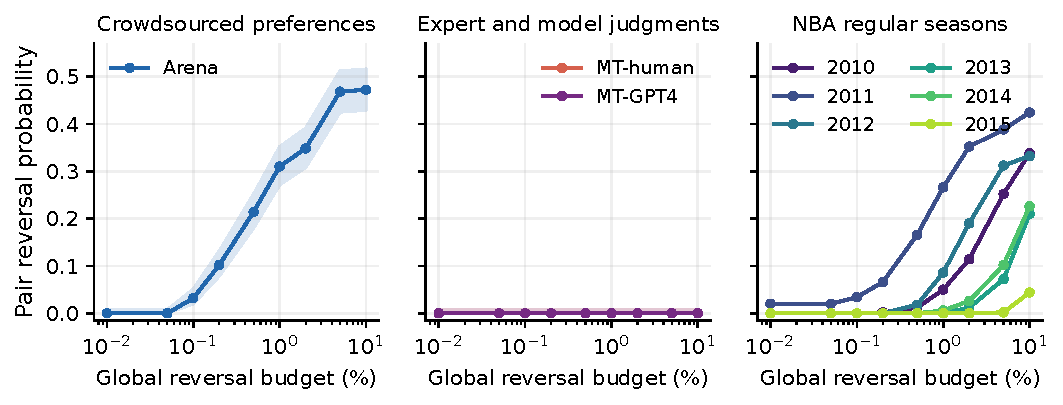
\includegraphics[width=\linewidth]{figures/random.pdf}
\caption{Leading-pair reversal under uniform decisive-outcome noise. Each point uses \num{Repeats} independent permutations. Shading shows pointwise Wilson 95\% Monte Carlo intervals for Arena and MT-Bench; NBA season curves are separate, without shaded intervals for readability. Small datasets round several small fractions to the same integer budget.}
\label{fig:random}
\end{figure}
At a global 1\% noise budget, Arena's original leading pair reverses in 31.0\% of runs (Wilson interval 27.1--35.2\%). Neither full MT-Bench panel reverses in any of the \num{Repeats} runs, whose Wilson upper limit is 0.8\%. Even at 10\% random reversals, neither full MT-Bench leading pair reverses in the observed runs. This is conditional simulation evidence, not proof that their reversal probability is zero. The NBA seasons vary substantially at the same fractions (Figure~\ref{fig:random}). The point-order threshold alone therefore does not describe a board's response to unselected label noise.

Small changes can also disturb less prominent ranks without removing the winner. At 1\% random noise, mean normalized Kendall discordance in Arena is 0.0115 despite its much larger leading-pair reversal probability. Conversely, full MT-human has occasional lower-rank changes at that budget with no winner change. Appendix~\ref{app:extra} reports both endpoints and empirical discordance ranges. These statistics measure distinct aspects of stability and should not be substituted for one another.

\subsection{Exposure changes the cross-design comparison}
\begin{figure}[t]
\centering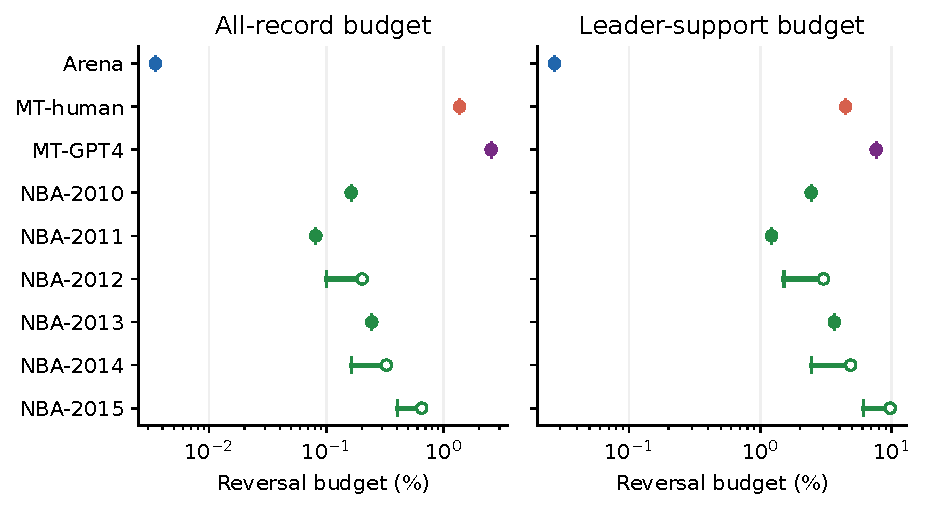
\includegraphics[width=\linewidth]{figures/normalization.pdf}
\caption{The same leading-pair count bounds under two denominators. Filled circles are exact minima; open circles are feasible upper bounds, with a segment to the certified lower bound. Leader support includes ties and remains fixed at the original dataset. The two scales describe exposure, not equal corruption effort.}
\label{fig:normalization}
\end{figure}
On the global scale, the MT-GPT4 leading-pair minimum is \num{MTGPTFourGlobalPct}\%, while every NBA constructed leading-pair budget is below 1\% (Table~\ref{tab:thresholds}). But GPT-4 contributes \num{MTGPTFourLeaderN} of \num{MTGPTFourN} MT-GPT4 records, compared with \num{NBA2015LeaderN} of \num{NBA2015N} games for the 2015 NBA leader. The same MT-GPT4 threshold is \num{MTGPTFourLeaderPct}\% of leader support; the 2015 NBA pair construction is \num{NBA2015LeaderPct}\%. The ordering of these \emph{upper/construction percentages} changes, while their certified intervals on the leader scale overlap. We therefore cannot conclude that NBA-2015 is intrinsically more robust. We can conclude that a global percentage alone exaggerates how comparable the supporting evidence is across these boards.

Arena remains unusually close under either scale, but that is a statement about this snapshot and pair. Within its top ten, adjacent-pair constructions range from \num{ArenaK} to \num{ArenaAdjacentMax} edits. Across all panels, including matched controls, the lower bound and feasible construction agree on \num{AdjacentTight} of \num{AdjacentCount} queried adjacent pairs. A single winner threshold consequently omits substantial within-board heterogeneity.

\subsection{Matched judgments and modeling controls}
\begin{table}[t]
\caption{Identical MT-Bench comparison schedules, one human judgment per common key, main seed. Both leading-pair minima are exact. Bootstrap intervals resample questions.}
\label{tab:matched}
\centering\small\begin{tabular}{lrrrrr}
\toprule
Panel & $N$ & $\widehat\Delta$ & Bootstrap 95\% interval & $K^*$ & $100K^*/N$ \\
\midrule
Matched-human & 1,814 & 0.283 & [0.066, 0.496] & 20 & 1.103 \\
Matched-GPT4 & 1,814 & 0.759 & [0.441, 1.107] & 42 & 2.315 \\
\bottomrule
\end{tabular}

\end{table}
Under the matched schedule, the human threshold is \num{MatchedhumanK} and the GPT-4 threshold is \num{MatchedGPTFourK} (Table~\ref{tab:matched}); their gaps also differ. Over \num{MatchedRepeats} selections of the human annotator per key, the human construction has median \num{MatchedHumanMedian} and observed range \num{MatchedHumanMin}--\num{MatchedHumanMax}. The matched GPT-4 dataset is unchanged across those selections. This controls several schedule differences, but does not prove a judge-design effect: the GPT-4 judge evaluates GPT-4's own responses, and greater score separation could reflect self-preference or a different rubric rather than greater accuracy \citep{zheng2023judge}.

Recomputed and static influence have the same leading-pair counts in every studied panel; restricting candidates to incident comparisons also leaves those counts unchanged. This is partly expected when the direct-win relaxation is attainable. It does not imply that remote comparisons never matter in other schedules. First-order counts match the exact-refit prefix in \num{AdjacentExactPrediction} of \num{AdjacentCount} adjacent-pair queries, with mean absolute count error \num{AdjacentMAE} and maximum \num{AdjacentMaxError}. Approximation accuracy is useful for finding edits, but is not an optimality certificate.

The modeling controls materially qualify the strongest-looking result. Arena's threshold becomes 1 at $\lambda=0.1$ and 11 at $\lambda=10$; dropping ties reverses the \emph{original} leading pair before any edit. The full MT-Bench thresholds remain 46 and 61 under these ridge changes, but dropping ties reduces them to 42 and 40, respectively, on the smaller decisive-only datasets. These are distinct estimands, not competing ways to estimate one immutable number. Adding a fitted home effect to each NBA season leaves the reported leading-pair construction counts unchanged; the theorem is not applied to those covariate fits. Deletion needs 3, 92, and 144 records for Arena, MT-human, and MT-GPT4 under its own static path. Appendix~\ref{app:extra} reports all controls, including the weaker curvature-only lower bound.

\section{Discussion, limitations, and responsible use}
\label{sec:limitations}
The defensible conclusion is conditional: in these reconstructed fixed-schedule boards, targeted edits can be much more effective than random noise, but a tiny reversal can concern an already unresolved order. We recommend reporting a certified interval or a clearly labeled feasible budget, the original gap with an uncertainty scale, and both global and participant-support fractions. A robust leading ordering can coexist with unstable lower ranks. A stable model-judge board can encode a systematic evaluation preference.

The finite-edit result is specific. It assumes standard item-only ridge BT, positive diagonal regularization, fixed comparison weights, and unit reversals of decisive labels. It does not cover arbitrary judge or home covariates, adaptive scheduling, new comparisons, removal of records, tie corruption, or corruption restricted by user identity. After direct-win capacity is exhausted the relaxation can be unattainable, as in several NBA seasons; the remaining count intervals are not silently resolved by a heuristic. The conservative analytic proofs are not machine-verified floating-point certificates.

The empirical comparison is descriptive rather than causal. There is one historical Arena snapshot and one small MT-Bench question collection; the NBA seasons are related cohorts in one sport. Model identities, sample sizes, margins, schedules, and stakes differ. Question clustering handles within-question dependence but not all shared-annotator effects; Arena lacks usable user clusters here, and game resampling ignores temporal, roster, and schedule dependence. Selection of top pairs also makes the bootstrap intervals descriptive. No interval estimates a universal population adversarial budget. We did not measure calibration, factual correctness, fairness, or the validity of the underlying judgments, nor run live attacks or evaluate defenses.

The audit can support more cautious leaderboard communication, but the edit-selection code could also inform manipulation. Its scope is offline analysis of public historical outcomes. We made no platform submissions or participant contacts, and release no conversation text or user profiles. The intended use is to audit uncertainty and evidence concentration, with qualified count bounds rather than assertions about deployed-system security. An OpenAI Codex assistant developed the methods, wrote and ran the code, inspected the results, and drafted the manuscript. No paid model calls generated judgments or experimental measurements; all reported evidence comes from the supplied public-data snapshots and actual CPU runs. This disclosure is essential to interpreting the artifact's provenance, and is not a substitute for independent scientific review.

\clearpage
\bibliographystyle{plainnat}
\bibliography{references}

\clearpage
\appendix
\section{Proofs and scope of the certificates}
\label{app:proof}
\subsection{Maximum principle and direct-transfer domination}
\begin{lemma}[Endpoint extrema]
\label{lem:maximum}
For $H=L_w+\lambda I$ with $L_w$ a symmetric graph Laplacian, nonnegative weights, and $\lambda>0$, let $v=H^{-1}(e_i-e_j)$ for $i\ne j$. Then $v_i=\max_m v_m>0$ and $v_j=\min_m v_m<0$.
\end{lemma}
\begin{proof}
Since $H\mathbf 1=\lambda\mathbf 1$, we have $\sum_m v_m=0$. Also $v\ne0$, so its maximum is positive and minimum is negative. If a positive maximum occurred at a node $m\ne i$, then
\begin{equation}
 (Hv)_m=\lambda v_m+\sum_q w_{mq}(v_m-v_q)>0.\label{eq:maxproof}
\end{equation}
This contradicts $(e_i-e_j)_m\le0$. Thus the maximum is attained only at $i$. The corresponding argument at a negative minimum shows it is attained only at $j$. Connectivity is not needed because ridge is positive at every node.
\end{proof}

\begin{proof}[Proof of Theorem~\ref{thm:direct}]
Equation~\eqref{eq:model} has Hessian
\begin{equation}
 H(\theta)=\sum_r\sigma(x_r^\top\theta)[1-\sigma(x_r^\top\theta)]x_rx_r^\top+\lambda I.\label{eq:hessian}
\end{equation}
It is a positive definite weighted Laplacian plus ridge, independent of outcomes at a fixed $\theta$. Its smallest eigenvalue is at least $\lambda$, so adding any linear term preserves coercivity, strong convexity, and a unique smooth optimizer.

Write $b_E=\sum_{q=1}^k u_q$, where every $u_q=e_{w_q}-e_{l_q}$. For $s\in[0,1]$, let $b(s)=(1-s)b_E+s k c$ and define $\theta(s)$ by $\nabla F(\theta(s))+b(s)=0$. Implicit differentiation yields
\begin{equation}
 \frac{d}{ds}c^\top\theta(s)
  =-v(s)^\top(kc-b_E),\qquad v(s)=H(\theta(s))^{-1}c.\label{eq:interpolation}
\end{equation}
By Lemma~\ref{lem:maximum}, $v(s)^\top u_q\le v_i(s)-v_j(s)=v(s)^\top c$. Therefore the derivative in Eq.~\eqref{eq:interpolation} is nonpositive. Integrating from zero to one proves Eq.~\eqref{eq:domination}. This step is why the argument is finite-edit rather than a first-order extrapolation at $\hat\theta$.

Along $tc$, implicit differentiation gives $d(c^\top\theta_c(t))/dt=-c^\top H(\theta_c(t))^{-1}c<0$. The integer crossing in Eq.~\eqref{eq:virtual} exists: the non-ridge gradient is bounded for a fixed finite schedule, whereas the ridge estimating equation implies $\theta_c(t)=-tc/\lambda+O(1)$ as $t\to\infty$. If $k<L_c$, the virtual gap is nonnegative, hence so is the gap for every feasible $k$-edit set. If $W_{ij}\ge L_c$, reversing $L_c$ distinct original $i$-over-$j$ wins yields exactly the linear term $L_c c$ and crosses. This proves both the bound and attainability.
\end{proof}

This theorem concerns the fixed queried contrast, not all ranks simultaneously. For original-winner loss, a strict reversal with any rival suffices, so taking the minimum over all rivals establishes Eq.~\eqref{eq:winner}. Upper/lower equality can also establish exactness without direct-capacity attainment. For example, NBA-2013 has direct capacity 2, pair lower bound 3, and a feasible three-edit construction. Bounds across rivals are recomputed from the original data, not from an already edited board.

\subsection{A generic curvature bound used as a comparison}
\label{app:curvature}
We also implemented a less specialized finite-edit bound to quantify the benefit of exploiting the item-comparison structure. Let $H_0=H(\hat\theta)$, $a=\max_r\|x_r\|_{H_0^{-1}}$, and $\rho=\hat\Delta/\|c\|_{H_0^{-1}}$. Sort the norms of eligible records in descending order and let $S_k$ be the sum of the largest $k$. Then
\begin{equation}
 S_k < \frac{1-e^{-a\rho}}{a}\quad\Longrightarrow\quad
 c^\top\hat\theta_E>0\text{ for every }|E|\le k.\label{eq:curv}
\end{equation}
To prove it, the logistic curvature $w(z)=\sigma(z)(1-\sigma(z))$ obeys $|d\log w(z)/dz|\le1$. For $d=\theta-\hat\theta$ and $R=\|d\|_{H_0}$, Cauchy--Schwarz gives $|x_r^\top d|\le aR$, hence $H(\hat\theta+u d)\succeq e^{-uaR}H_0$ for $u\in[0,1]$ (the ridge term also satisfies this inequality). At the edited optimum, with $q=\|b_E\|_{H_0^{-1}}$,
\begin{equation}
 Rq\ \ge -d^\top b_E
 =\int_0^1d^\top H(\hat\theta+u d)d\,du
 \ge \frac{R}{a}(1-e^{-aR}).\label{eq:radial}
\end{equation}
For $R>0$, Eq.~\eqref{eq:radial} and $q\le S_k$ imply $R<\rho$ under Eq.~\eqref{eq:curv}. Such a displacement cannot reach the contrast-zero hyperplane. The $R=0$ case is immediate. Code adds the inverse-Hessian norm of any initial numerical gradient residual to $S_k$ and a strict numerical guard. Table~\ref{tab:methods} reports this certificate as a lower bound $L_{\rm curv}=k_{\rm safe}+1$ on the minimum count, not as an attack. Failure to certify even one edit is not evidence that one edit suffices.

\section{Supplementary measurements}
\label{app:extra}
\begin{table}[h]
\caption{Constructed leading-pair thresholds and lower bounds. $W_{\ell r}$ is direct-win capacity; $L_{\rm dir}$ is Theorem~\ref{thm:direct}'s necessary count; $L_{\rm curv}$ is the curvature-only necessary count. Adaptive and incident columns are feasible flip constructions. Delete uses its own operation and ordering and has no direct-transfer certificate.}
\label{tab:methods}
\centering\small\begin{tabular}{lrrrrrrr}
\toprule
Panel & $W_{\ell r}$ & $L_{\rm dir}$ & $U$ & $L_{\rm curv}$ & Adaptive & Incident & Delete \\
\midrule
Arena & 31 & 2 & 2 & 1 & 2 & 2 & 3 \\
MT-human & 91 & 46 & 46 & 31 & 46 & 46 & 92 \\
MT-GPT4 & 75 & 61 & 61 & 27 & 61 & 61 & 144 \\
NBA-2010 & 2 & 2 & 2 & 1 & 2 & 2 & 3 \\
NBA-2011 & 1 & 1 & 1 & 1 & 1 & 1 & 2 \\
NBA-2012 & 0 & 1 & 2 & 1 & 2 & 2 & 2 \\
NBA-2013 & 2 & 3 & 3 & 2 & 3 & 3 & 5 \\
NBA-2014 & 0 & 2 & 4 & 2 & 4 & 4 & 4 \\
NBA-2015 & 1 & 5 & 8 & 3 & 8 & 8 & 9 \\
Matched-human & 51 & 20 & 20 & 14 & 20 & 20 & 39 \\
Matched-GPT4 & 55 & 42 & 42 & 20 & 42 & 42 & 96 \\
\bottomrule
\end{tabular}

\end{table}

\begin{table}[h]
\caption{Uniform noise at 1\% of all records. Pair and winner columns are event percentages across \num{Repeats} permutations. Wilson intervals measure Monte Carlo error for the pair probability. $D_K$ is discordant item pairs divided by $\binom M2$; its central range is empirical across perturbations, not a confidence interval for its mean.}
\label{tab:random}
\centering\scriptsize\begin{tabular}{lrrrrr}
\toprule
Panel & Pair (\%) & Wilson 95\% interval & Winner (\%) & Mean $D_K$ & Central 95\% $D_K$ \\
\midrule
Arena & 31.0 & [27.1, 35.2] & 31.0 & 0.0115 & [0.0069, 0.0174] \\
MT-human & 0.0 & [0.0, 0.8] & 0.0 & 0.0005 & [0.0000, 0.0000] \\
MT-GPT4 & 0.0 & [0.0, 0.8] & 0.0 & 0.0000 & [0.0000, 0.0000] \\
NBA-2010 & 5.0 & [3.4, 7.3] & 7.8 & 0.0222 & [0.0092, 0.0345] \\
NBA-2011 & 26.6 & [22.9, 30.6] & 26.6 & 0.0174 & [0.0069, 0.0288] \\
NBA-2012 & 8.6 & [6.4, 11.4] & 9.0 & 0.0234 & [0.0092, 0.0368] \\
NBA-2013 & 0.0 & [0.0, 0.8] & 0.0 & 0.0185 & [0.0092, 0.0299] \\
NBA-2014 & 0.6 & [0.2, 1.7] & 0.6 & 0.0147 & [0.0046, 0.0253] \\
NBA-2015 & 0.0 & [0.0, 0.8] & 0.0 & 0.0201 & [0.0092, 0.0322] \\
Matched-human & 0.0 & [0.0, 0.8] & 0.0 & 0.0000 & [0.0000, 0.0000] \\
Matched-GPT4 & 0.0 & [0.0, 0.8] & 0.0 & 0.0000 & [0.0000, 0.0000] \\
\bottomrule
\end{tabular}

\end{table}

\begin{figure}[h]
\centering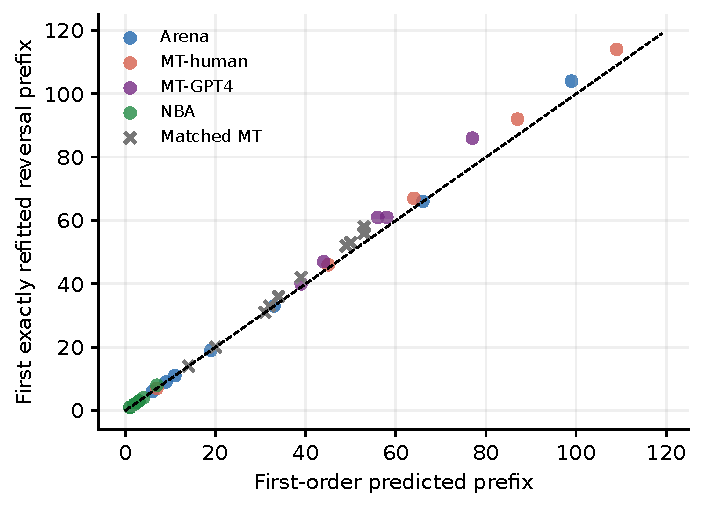
\includegraphics[width=.8\linewidth]{figures/influence.pdf}
\caption{Initial influence prediction versus exactly refitted first crossing along its sorted path. These \num{AdjacentCount} queries cover all adjacent pairs among the original top ten (or all six models for MT-Bench), including matched controls. Coincident markers are not jittered. Prediction agreement does not establish global optimality.}
\label{fig:influence}
\end{figure}

\clearpage
\begin{table}[p]
\caption{All modeling controls. The original main-fit pair is held fixed, so a zero threshold means the alternative modeling choice already reverses it. Ridge is on the summed loss. Drop-ties changes the observation count and loss weights; these counts are not percentages on the original denominator. Home-covariate fits are upper-bound constructions only.}
\label{tab:ablations}
\centering\scriptsize\begin{tabular}{lllrr}
\toprule
Panel & Variant & Fitted winner & Original-pair gap & $U$ \\
\midrule
Arena & ridge-0.1 & gpt-4-1106-preview & 0.0042 & 1 \\
Arena & ridge-10 & gpt-4-1106-preview & 0.0436 & 11 \\
Arena & drop-ties & gpt-4-0125-preview & -0.0226 & 0 \\
MT-human & ridge-0.1 & gpt-4 & 0.3781 & 46 \\
MT-human & ridge-10 & gpt-4 & 0.3574 & 46 \\
MT-human & drop-ties & gpt-4 & 0.5270 & 42 \\
MT-GPT4 & ridge-0.1 & gpt-4 & 0.8198 & 61 \\
MT-GPT4 & ridge-10 & gpt-4 & 0.7245 & 61 \\
MT-GPT4 & drop-ties & gpt-4 & 1.0645 & 40 \\
NBA-2010 & ridge-0.1 & CLE & 0.1272 & 2 \\
NBA-2010 & ridge-10 & CLE & 0.0697 & 2 \\
NBA-2010 & home-covariate & CLE & 0.1272 & 2 \\
NBA-2011 & ridge-0.1 & SAS & 0.0729 & 1 \\
NBA-2011 & ridge-10 & SAS & 0.0170 & 1 \\
NBA-2011 & home-covariate & SAS & 0.0668 & 1 \\
NBA-2012 & ridge-0.1 & SAS & 0.1278 & 2 \\
NBA-2012 & ridge-10 & SAS & 0.0347 & 1 \\
NBA-2012 & home-covariate & SAS & 0.1037 & 2 \\
NBA-2013 & ridge-0.1 & MIA & 0.3044 & 3 \\
NBA-2013 & ridge-10 & MIA & 0.1740 & 3 \\
NBA-2013 & home-covariate & MIA & 0.2909 & 3 \\
NBA-2014 & ridge-0.1 & SAS & 0.2016 & 4 \\
NBA-2014 & ridge-10 & SAS & 0.1090 & 4 \\
NBA-2014 & home-covariate & SAS & 0.1946 & 4 \\
NBA-2015 & ridge-0.1 & GSW & 0.6122 & 8 \\
NBA-2015 & ridge-10 & GSW & 0.2865 & 7 \\
NBA-2015 & home-covariate & GSW & 0.5579 & 8 \\
Matched-human & ridge-0.1 & gpt-4 & 0.2865 & 20 \\
Matched-human & ridge-10 & gpt-4 & 0.2561 & 20 \\
Matched-human & drop-ties & gpt-4 & 0.4278 & 19 \\
Matched-GPT4 & ridge-0.1 & gpt-4 & 0.7722 & 42 \\
Matched-GPT4 & ridge-10 & gpt-4 & 0.6550 & 42 \\
Matched-GPT4 & drop-ties & gpt-4 & 0.9882 & 28 \\
\bottomrule
\end{tabular}

\end{table}
\clearpage
\subsection{All adjacent-pair queries}
The following tables give the fitted pair, baseline gap, certified optimal-count interval, and first-order prefix prediction for every query. Rows are selected by the original ranking and are descriptive, without multiplicity-adjusted inferential claims. Original model identifiers are preserved.
\newcommand{\adjtable}[1]{\begin{table}[ht]\centering\scriptsize\caption{Adjacent pairs: #1.}\input{tables/adjacent_#1}\end{table}}
\adjtable{Arena}
\adjtable{MT-human}
\adjtable{MT-GPT4}
\adjtable{NBA-2010}
\adjtable{NBA-2011}
\adjtable{NBA-2012}
\adjtable{NBA-2013}
\adjtable{NBA-2014}
\adjtable{NBA-2015}
\adjtable{Matched-human}
\adjtable{Matched-GPT4}
\clearpage

\section{Reproduction, provenance, and research boundaries}
\label{app:repro}
\paragraph{Environment and commands.}
The artifact includes pinned Python dependencies, all scripts, generated CSV/JSON results, and the official NeurIPS 2026 style and checklist. It uses Python 3.11.2, NumPy 2.4.6, SciPy 1.17.1, pandas 3.1.0, PyArrow 26.0.0, and Matplotlib 3.11.2. CPU linear algebra is restricted to one thread; no GPU, training, or paid API is used. From the project root, \texttt{make reproduce} downloads/checks the data, runs verification, main and winner experiments, validates result witnesses, regenerates all displays, and compiles the PDF. The initial main run before the direct-transfer addition took 91.6\,s; the complete main run reported in this manuscript took \num{MainSeconds}\,s. The data download, preliminary fits, verification, and reporting are additional work, documented in the research log. No numerical fit failed in the reported run. The reproduction script records fresh timings rather than assuming identical wall time.

\paragraph{Display provenance.}
All tables and figures are generated by \texttt{src/report.py}. Table~\ref{tab:data} uses \texttt{summary.csv}; Table~\ref{tab:thresholds} uses \texttt{summary.csv} and \texttt{winner.csv}; Table~\ref{tab:matched} uses \texttt{summary.csv}. Figure~\ref{fig:random} and Table~\ref{tab:random} use \texttt{random.csv}; Figure~\ref{fig:normalization} uses \texttt{summary.csv}; Figure~\ref{fig:influence} and all adjacent-pair tables use \texttt{adjacent.csv}. Table~\ref{tab:methods} uses \texttt{summary.csv}; Table~\ref{tab:ablations} uses \texttt{ablations.csv}. These files are produced by \texttt{src/experiment.py}, except the all-rival winner audit, produced by \texttt{src/winner.py}. Text macros come from the same results, and raw bootstrap gaps and edit witnesses are retained. The artifact README gives a complete file map.

\paragraph{Frozen data and licenses.}
The manifest records full URLs, versions, sizes, and SHA-256 digests. Arena uses dataset commit \texttt{18c298340948c0e7f7727399fd459cca6ce0ca6f} (Apache-2.0). Both MT-Bench files use \texttt{f7d2896d2cc5d80f8b55c2bbc722613555233c25} (CC-BY-4.0). NBA uses repository commit \texttt{4c1ff5e3aef1816ae04af63218015066e186c147} (CC-BY-4.0), credited to FiveThirtyEight and its game-data source Basketball-Reference as stated in the repository. Dataset cards and the NBA license are preserved locally. The raw data remain in \texttt{data/raw/} and are excluded from the submission archive. Reproduction downloads the same public snapshots, without accounts. No large optional dataset was needed.

\paragraph{Restricted reading and independent work.}
We did not conduct general literature or web searches, follow citation links, inspect contemporary leaderboard analyses, or attempt to identify the excluded work. We directly downloaded and consulted five permitted starting papers (Arena, MT-Bench, influence functions, automatic finite-sample robustness, and vote rigging), plus the named datasets' documentation and official conference formatting/ethics pages. We did not open the other supplied starting papers. No known prohibited material was encountered. The access log records requested URLs and reading scope, including unsuccessful template URLs. Restricting access in this way limits the completeness of related-work coverage and prevents any claim of exhaustive novelty priority.

\clearpage
\section*{NeurIPS Paper Checklist}




\begin{enumerate}

\item {\bf Claims}
    \item[] Question: Do the main claims made in the abstract and introduction accurately reflect the paper's contributions and scope?
    \item[] Answer: \answerYes{}
    \item[] Justification: Sections 1 and 5 distinguish exact counts, bounded counts, uncertainty, and the fixed-schedule scope.
    \item[] Guidelines:
    \begin{itemize}
        \item The answer \answerNA{} means that the abstract and introduction do not include the claims made in the paper.
        \item The abstract and/or introduction should clearly state the claims made, including the contributions made in the paper and important assumptions and limitations. A \answerNo{} or \answerNA{} answer to this question will not be perceived well by the reviewers. 
        \item The claims made should match theoretical and experimental results, and reflect how much the results can be expected to generalize to other settings. 
        \item It is fine to include aspirational goals as motivation as long as it is clear that these goals are not attained by the paper. 
    \end{itemize}

\item {\bf Limitations}
    \item[] Question: Does the paper discuss the limitations of the work performed by the authors?
    \item[] Answer: \answerYes{}
    \item[] Justification: Section 6 discusses model assumptions, dataset coverage, dependence, selection, judge bias, and offline access.
    \item[] Guidelines:
    \begin{itemize}
        \item The answer \answerNA{} means that the paper has no limitation while the answer \answerNo{} means that the paper has limitations, but those are not discussed in the paper. 
        \item The authors are encouraged to create a separate ``Limitations'' section in their paper.
        \item The paper should point out any strong assumptions and how robust the results are to violations of these assumptions (e.g., independence assumptions, noiseless settings, model well-specification, asymptotic approximations only holding locally). The authors should reflect on how these assumptions might be violated in practice and what the implications would be.
        \item The authors should reflect on the scope of the claims made, e.g., if the approach was only tested on a few datasets or with a few runs. In general, empirical results often depend on implicit assumptions, which should be articulated.
        \item The authors should reflect on the factors that influence the performance of the approach. For example, a facial recognition algorithm may perform poorly when image resolution is low or images are taken in low lighting. Or a speech-to-text system might not be used reliably to provide closed captions for online lectures because it fails to handle technical jargon.
        \item The authors should discuss the computational efficiency of the proposed algorithms and how they scale with dataset size.
        \item If applicable, the authors should discuss possible limitations of their approach to address problems of privacy and fairness.
        \item While the authors might fear that complete honesty about limitations might be used by reviewers as grounds for rejection, a worse outcome might be that reviewers discover limitations that aren't acknowledged in the paper. The authors should use their best judgment and recognize that individual actions in favor of transparency play an important role in developing norms that preserve the integrity of the community. Reviewers will be specifically instructed to not penalize honesty concerning limitations.
    \end{itemize}

\item {\bf Theory assumptions and proofs}
    \item[] Question: For each theoretical result, does the paper provide the full set of assumptions and a complete (and correct) proof?
    \item[] Answer: \answerYes{}
    \item[] Justification: Theorem 1 states the assumptions; Appendix A gives the complete maximum-principle and interpolation proofs, plus the curvature-bound proof.
    \item[] Guidelines:
    \begin{itemize}
        \item The answer \answerNA{} means that the paper does not include theoretical results. 
        \item All the theorems, formulas, and proofs in the paper should be numbered and cross-referenced.
        \item All assumptions should be clearly stated or referenced in the statement of any theorems.
        \item The proofs can either appear in the main paper or the supplemental material, but if they appear in the supplemental material, the authors are encouraged to provide a short proof sketch to provide intuition. 
        \item Inversely, any informal proof provided in the core of the paper should be complemented by formal proofs provided in appendix or supplemental material.
        \item Theorems and Lemmas that the proof relies upon should be properly referenced. 
    \end{itemize}

    \item {\bf Experimental result reproducibility}
    \item[] Question: Does the paper fully disclose all the information needed to reproduce the main experimental results of the paper to the extent that it affects the main claims and/or conclusions of the paper (regardless of whether the code and data are provided or not)?
    \item[] Answer: \answerYes{}
    \item[] Justification: Sections 3--4 and Appendix C specify the objective, eligibility, endpoints, controls, seeds, resampling, and exact reproduction commands.
    \item[] Guidelines:
    \begin{itemize}
        \item The answer \answerNA{} means that the paper does not include experiments.
        \item If the paper includes experiments, a \answerNo{} answer to this question will not be perceived well by the reviewers: Making the paper reproducible is important, regardless of whether the code and data are provided or not.
        \item If the contribution is a dataset and\slash or model, the authors should describe the steps taken to make their results reproducible or verifiable. 
        \item Depending on the contribution, reproducibility can be accomplished in various ways. For example, if the contribution is a novel architecture, describing the architecture fully might suffice, or if the contribution is a specific model and empirical evaluation, it may be necessary to either make it possible for others to replicate the model with the same dataset, or provide access to the model. In general. releasing code and data is often one good way to accomplish this, but reproducibility can also be provided via detailed instructions for how to replicate the results, access to a hosted model (e.g., in the case of a large language model), releasing of a model checkpoint, or other means that are appropriate to the research performed.
        \item While NeurIPS does not require releasing code, the conference does require all submissions to provide some reasonable avenue for reproducibility, which may depend on the nature of the contribution. For example
        \begin{enumerate}
            \item If the contribution is primarily a new algorithm, the paper should make it clear how to reproduce that algorithm.
            \item If the contribution is primarily a new model architecture, the paper should describe the architecture clearly and fully.
            \item If the contribution is a new model (e.g., a large language model), then there should either be a way to access this model for reproducing the results or a way to reproduce the model (e.g., with an open-source dataset or instructions for how to construct the dataset).
            \item We recognize that reproducibility may be tricky in some cases, in which case authors are welcome to describe the particular way they provide for reproducibility. In the case of closed-source models, it may be that access to the model is limited in some way (e.g., to registered users), but it should be possible for other researchers to have some path to reproducing or verifying the results.
        \end{enumerate}
    \end{itemize}


\item {\bf Open access to data and code}
    \item[] Question: Does the paper provide open access to the data and code, with sufficient instructions to faithfully reproduce the main experimental results, as described in supplemental material?
    \item[] Answer: \answerYes{}
    \item[] Justification: The accompanying artifact includes all code and generated results. Frozen public data URLs, full checksums, dependency versions, and acquisition scripts are supplied; raw data are downloaded separately.
    \item[] Guidelines:
    \begin{itemize}
        \item The answer \answerNA{} means that paper does not include experiments requiring code.
        \item Please see the NeurIPS code and data submission guidelines (\url{https://neurips.cc/public/guides/CodeSubmissionPolicy}) for more details.
        \item While we encourage the release of code and data, we understand that this might not be possible, so \answerNo{} is an acceptable answer. Papers cannot be rejected simply for not including code, unless this is central to the contribution (e.g., for a new open-source benchmark).
        \item The instructions should contain the exact command and environment needed to run to reproduce the results. See the NeurIPS code and data submission guidelines (\url{https://neurips.cc/public/guides/CodeSubmissionPolicy}) for more details.
        \item The authors should provide instructions on data access and preparation, including how to access the raw data, preprocessed data, intermediate data, and generated data, etc.
        \item The authors should provide scripts to reproduce all experimental results for the new proposed method and baselines. If only a subset of experiments are reproducible, they should state which ones are omitted from the script and why.
        \item At submission time, to preserve anonymity, the authors should release anonymized versions (if applicable).
        \item Providing as much information as possible in supplemental material (appended to the paper) is recommended, but including URLs to data and code is permitted.
    \end{itemize}


\item {\bf Experimental setting/details}
    \item[] Question: Does the paper specify all the training and test details (e.g., data splits, hyperparameters, how they were chosen, type of optimizer) necessary to understand the results?
    \item[] Answer: \answerYes{}
    \item[] Justification: Sections 3--4 specify all settings; no hyperparameter search, training/test split, or fitted prediction benchmark is used.
    \item[] Guidelines:
    \begin{itemize}
        \item The answer \answerNA{} means that the paper does not include experiments.
        \item The experimental setting should be presented in the core of the paper to a level of detail that is necessary to appreciate the results and make sense of them.
        \item The full details can be provided either with the code, in appendix, or as supplemental material.
    \end{itemize}

\item {\bf Experiment statistical significance}
    \item[] Question: Does the paper report error bars suitably and correctly defined or other appropriate information about the statistical significance of the experiments?
    \item[] Answer: \answerYes{}
    \item[] Justification: Sections 3.3 and 5 explain question-cluster/record/game bootstrap intervals and conditional Monte Carlo Wilson intervals. Deterministic finite-dataset attack counts have no artificial error bars; descriptive and selection limitations are stated.
    \item[] Guidelines:
    \begin{itemize}
        \item The answer \answerNA{} means that the paper does not include experiments.
        \item The authors should answer \answerYes{} if the results are accompanied by error bars, confidence intervals, or statistical significance tests, at least for the experiments that support the main claims of the paper.
        \item The factors of variability that the error bars are capturing should be clearly stated (for example, train/test split, initialization, random drawing of some parameter, or overall run with given experimental conditions).
        \item The method for calculating the error bars should be explained (closed form formula, call to a library function, bootstrap, etc.)
        \item The assumptions made should be given (e.g., Normally distributed errors).
        \item It should be clear whether the error bar is the standard deviation or the standard error of the mean.
        \item It is OK to report 1-sigma error bars, but one should state it. The authors should preferably report a 2-sigma error bar than state that they have a 96\% CI, if the hypothesis of Normality of errors is not verified.
        \item For asymmetric distributions, the authors should be careful not to show in tables or figures symmetric error bars that would yield results that are out of range (e.g., negative error rates).
        \item If error bars are reported in tables or plots, the authors should explain in the text how they were calculated and reference the corresponding figures or tables in the text.
    \end{itemize}

\item {\bf Experiments compute resources}
    \item[] Question: For each experiment, does the paper provide sufficient information on the computer resources (type of compute workers, memory, time of execution) needed to reproduce the experiments?
    \item[] Answer: \answerYes{}
    \item[] Justification: Section 4 and Appendix C report CPU model, thread count, wall times, memory, and absence of GPU use; the research log records preliminary work.
    \item[] Guidelines:
    \begin{itemize}
        \item The answer \answerNA{} means that the paper does not include experiments.
        \item The paper should indicate the type of compute workers CPU or GPU, internal cluster, or cloud provider, including relevant memory and storage.
        \item The paper should provide the amount of compute required for each of the individual experimental runs as well as estimate the total compute. 
        \item The paper should disclose whether the full research project required more compute than the experiments reported in the paper (e.g., preliminary or failed experiments that didn't make it into the paper). 
    \end{itemize}
    
\item {\bf Code of ethics}
    \item[] Question: Does the research conducted in the paper conform, in every respect, with the NeurIPS Code of Ethics \url{https://neurips.cc/public/EthicsGuidelines}?
    \item[] Answer: \answerYes{}
    \item[] Justification: The official ethics guidelines were reviewed. Section 6 describes offline use of public licensed data, no participant contact or live manipulation, and exclusion of conversations from the release.
    \item[] Guidelines:
    \begin{itemize}
        \item The answer \answerNA{} means that the authors have not reviewed the NeurIPS Code of Ethics.
        \item If the authors answer \answerNo, they should explain the special circumstances that require a deviation from the Code of Ethics.
        \item The authors should make sure to preserve anonymity (e.g., if there is a special consideration due to laws or regulations in their jurisdiction).
    \end{itemize}


\item {\bf Broader impacts}
    \item[] Question: Does the paper discuss both potential positive societal impacts and negative societal impacts of the work performed?
    \item[] Answer: \answerYes{}
    \item[] Justification: Section 6 discusses more cautious leaderboard use and potential misuse of edit-selection code.
    \item[] Guidelines:
    \begin{itemize}
        \item The answer \answerNA{} means that there is no societal impact of the work performed.
        \item If the authors answer \answerNA{} or \answerNo, they should explain why their work has no societal impact or why the paper does not address societal impact.
        \item Examples of negative societal impacts include potential malicious or unintended uses (e.g., disinformation, generating fake profiles, surveillance), fairness considerations (e.g., deployment of technologies that could make decisions that unfairly impact specific groups), privacy considerations, and security considerations.
        \item The conference expects that many papers will be foundational research and not tied to particular applications, let alone deployments. However, if there is a direct path to any negative applications, the authors should point it out. For example, it is legitimate to point out that an improvement in the quality of generative models could be used to generate Deepfakes for disinformation. On the other hand, it is not needed to point out that a generic algorithm for optimizing neural networks could enable people to train models that generate Deepfakes faster.
        \item The authors should consider possible harms that could arise when the technology is being used as intended and functioning correctly, harms that could arise when the technology is being used as intended but gives incorrect results, and harms following from (intentional or unintentional) misuse of the technology.
        \item If there are negative societal impacts, the authors could also discuss possible mitigation strategies (e.g., gated release of models, providing defenses in addition to attacks, mechanisms for monitoring misuse, mechanisms to monitor how a system learns from feedback over time, improving the efficiency and accessibility of ML).
    \end{itemize}
    
\item {\bf Safeguards}
    \item[] Question: Does the paper describe safeguards that have been put in place for responsible release of data or models that have a high risk for misuse (e.g., pre-trained language models, image generators, or scraped datasets)?
    \item[] Answer: \answerNA{}
    \item[] Justification: No new high-risk model or scraped dataset is released. The artifact is an offline audit of existing public data; Section 6 states its misuse limitations and release scope.
    \item[] Guidelines:
    \begin{itemize}
        \item The answer \answerNA{} means that the paper poses no such risks.
        \item Released models that have a high risk for misuse or dual-use should be released with necessary safeguards to allow for controlled use of the model, for example by requiring that users adhere to usage guidelines or restrictions to access the model or implementing safety filters. 
        \item Datasets that have been scraped from the Internet could pose safety risks. The authors should describe how they avoided releasing unsafe images.
        \item We recognize that providing effective safeguards is challenging, and many papers do not require this, but we encourage authors to take this into account and make a best faith effort.
    \end{itemize}

\item {\bf Licenses for existing assets}
    \item[] Question: Are the creators or original owners of assets (e.g., code, data, models), used in the paper, properly credited and are the license and terms of use explicitly mentioned and properly respected?
    \item[] Answer: \answerYes{}
    \item[] Justification: Appendix C and the data manifest credit creators, preserve exact snapshots and dataset cards, and list Apache-2.0 and CC-BY-4.0 terms. The official template is preserved unchanged.
    \item[] Guidelines:
    \begin{itemize}
        \item The answer \answerNA{} means that the paper does not use existing assets.
        \item The authors should cite the original paper that produced the code package or dataset.
        \item The authors should state which version of the asset is used and, if possible, include a URL.
        \item The name of the license (e.g., CC-BY 4.0) should be included for each asset.
        \item For scraped data from a particular source (e.g., website), the copyright and terms of service of that source should be provided.
        \item If assets are released, the license, copyright information, and terms of use in the package should be provided. For popular datasets, \url{paperswithcode.com/datasets} has curated licenses for some datasets. Their licensing guide can help determine the license of a dataset.
        \item For existing datasets that are re-packaged, both the original license and the license of the derived asset (if it has changed) should be provided.
        \item If this information is not available online, the authors are encouraged to reach out to the asset's creators.
    \end{itemize}

\item {\bf New assets}
    \item[] Question: Are new assets introduced in the paper well documented and is the documentation provided alongside the assets?
    \item[] Answer: \answerYes{}
    \item[] Justification: The new code, result files, numerical witnesses, README, and display provenance map are included; data downloads remain separate and code licensing is explicit.
    \item[] Guidelines:
    \begin{itemize}
        \item The answer \answerNA{} means that the paper does not release new assets.
        \item Researchers should communicate the details of the dataset\slash code\slash model as part of their submissions via structured templates. This includes details about training, license, limitations, etc. 
        \item The paper should discuss whether and how consent was obtained from people whose asset is used.
        \item At submission time, remember to anonymize your assets (if applicable). You can either create an anonymized URL or include an anonymized zip file.
    \end{itemize}

\item {\bf Crowdsourcing and research with human subjects}
    \item[] Question: For crowdsourcing experiments and research with human subjects, does the paper include the full text of instructions given to participants and screenshots, if applicable, as well as details about compensation (if any)? 
    \item[] Answer: \answerNA{}
    \item[] Justification: No new crowdsourcing or human-participant interaction was conducted. Existing expert and crowd datasets are used for secondary analysis and credited in Section 4.
    \item[] Guidelines:
    \begin{itemize}
        \item The answer \answerNA{} means that the paper does not involve crowdsourcing nor research with human subjects.
        \item Including this information in the supplemental material is fine, but if the main contribution of the paper involves human subjects, then as much detail as possible should be included in the main paper. 
        \item According to the NeurIPS Code of Ethics, workers involved in data collection, curation, or other labor should be paid at least the minimum wage in the country of the data collector. 
    \end{itemize}

\item {\bf Institutional review board (IRB) approvals or equivalent for research with human subjects}
    \item[] Question: Does the paper describe potential risks incurred by study participants, whether such risks were disclosed to the subjects, and whether Institutional Review Board (IRB) approvals (or an equivalent approval/review based on the requirements of your country or institution) were obtained?
    \item[] Answer: \answerNA{}
    \item[] Justification: No participants were recruited, contacted, or assigned interventions. Only public historical records are analyzed; we do not claim a new IRB approval.
    \item[] Guidelines:
    \begin{itemize}
        \item The answer \answerNA{} means that the paper does not involve crowdsourcing nor research with human subjects.
        \item Depending on the country in which research is conducted, IRB approval (or equivalent) may be required for any human subjects research. If you obtained IRB approval, you should clearly state this in the paper. 
        \item We recognize that the procedures for this may vary significantly between institutions and locations, and we expect authors to adhere to the NeurIPS Code of Ethics and the guidelines for their institution. 
        \item For initial submissions, do not include any information that would break anonymity (if applicable), such as the institution conducting the review.
    \end{itemize}

\item {\bf Declaration of LLM usage}
    \item[] Question: Does the paper describe the usage of LLMs if it is an important, original, or non-standard component of the core methods in this research? Note that if the LLM is used only for writing, editing, or formatting purposes and does \emph{not} impact the core methodology, scientific rigor, or originality of the research, declaration is not required.
    %this research? 
    \item[] Answer: \answerYes{}
    \item[] Justification: Section 6 explicitly discloses that an OpenAI Codex assistant developed the method and code, ran the study, inspected results, and drafted the manuscript. LLM generation is not an experimental measurement.
    \item[] Guidelines:
    \begin{itemize}
        \item The answer \answerNA{} means that the core method development in this research does not involve LLMs as any important, original, or non-standard components.
        \item Please refer to our LLM policy in the NeurIPS handbook for what should or should not be described.
    \end{itemize}

\end{enumerate}
\end{document}
